\documentclass[9pt,a4paper]{article}
\usepackage[utf8]{inputenc}
\usepackage{url}

\usepackage{a4wide}
\usepackage{longtable}           % lange Tabellen
\usepackage{graphicx}
\usepackage{amsmath}
\usepackage{multirow}
\usepackage{enumerate}
\usepackage{listings}

\usepackage{nopageno}
\usepackage[margin=1cm]{geometry}



%\usepackage{fancyhdr}

%\bibliographystyle{alpha} % does not work as expected

%% \pagestyle{fancy}
%% %\fancyhf{}                              % bisherige Kopf- und Fusszeilen loeschen
%% %\fancyhead[R]{Nico Schottelius}            % rechter Kopfzeileneintrag
%% \fancyhead[R]{}
%% %\fancyhead[L]{Projekdokumentation}      % linker Kopfzeileneintrag
%% %\fancyhead[L]{\thepage}      % linker Kopfzeileneintrag
%% %\fancyfoot[C]{\thepage}                % Fusszeileneintrag (Seitenzahl zentriert)
%% \renewcommand{\headrulewidth}{0.4pt}  % Strichstaerke unter der Kopfzeile
% ----------------------------------------------------------------------------
% let's start
\begin{document}
\title{Bachelorarbeit Zusammenfassung\\
Development of a secure, peer-to-peer, decentralised
anonymous chat system}
\date{\today}
\author{Nico Schottelius (nico-zhaw.ch (o) schottelius.org)\\ZHAW}
% ----------------------------------------------------------------------------
\maketitle
% ----------------------------------------------------------------------------
% Grundlagen
Das Ziel dieser Bachelorarbeit ist es, ein Chat-Protokoll zu erstellen,
das sichere, anonyme Kommunikation ermöglicht. Aufgrund der einfachen
Angreifbarkeit zentraler Systeme wurde zusätzlich die Einschränkung
auf ein dezentrales System beschlossen. Anonyme Kommunikation ist im Vergleich
zur realen Welt im Internet schwieriger zu erreichen, da theorethisch
sämtliche Leitungen von einem Angreifer abgehört werden können. Daraus ergibt
sich, dass jede Nachricht geschützt sein muss, sowohl
gegen Betrachtung von einer
unzulässigen Person ("`Geheimhaltung"'), als auch gegen Veränderung.

%Vorgehensweise
Die Entwicklung der vorliegenden Arbeit ist durch das Spiral-Modell der 
Softwareentwicklung geprägt: Während zunächst ein Teil
des Chat-Protokolls definiert wurde, wurde im nächsten Arbeitsschritt 
diese Definition im Prototypen implementiert.
So konnten die Erfahrungen in der Implementation wieder direkt in die Definition
des Protokolls zurückfliessen.

%Ergebnisse 
Die vorliegende Arbeit präsentiert nicht nur eine vollständige
Definition des Chat-Protokolls und einen funktionsfähigen Prototypen, sondern
beinhaltet Analysen von Chat-Systemen und Kommunikationsprotokollen.
Insbesondere die Betrachtung der Anonymisierungssysteme, wie beispielsweise Tor
oder den Mix-Netzen, zeigt, dass das Thema anonyme Kommunikation bereits
seit langer Zeit in der Informatik mit verschiedensten Ansätzen behandelt
und diskutiert wird.

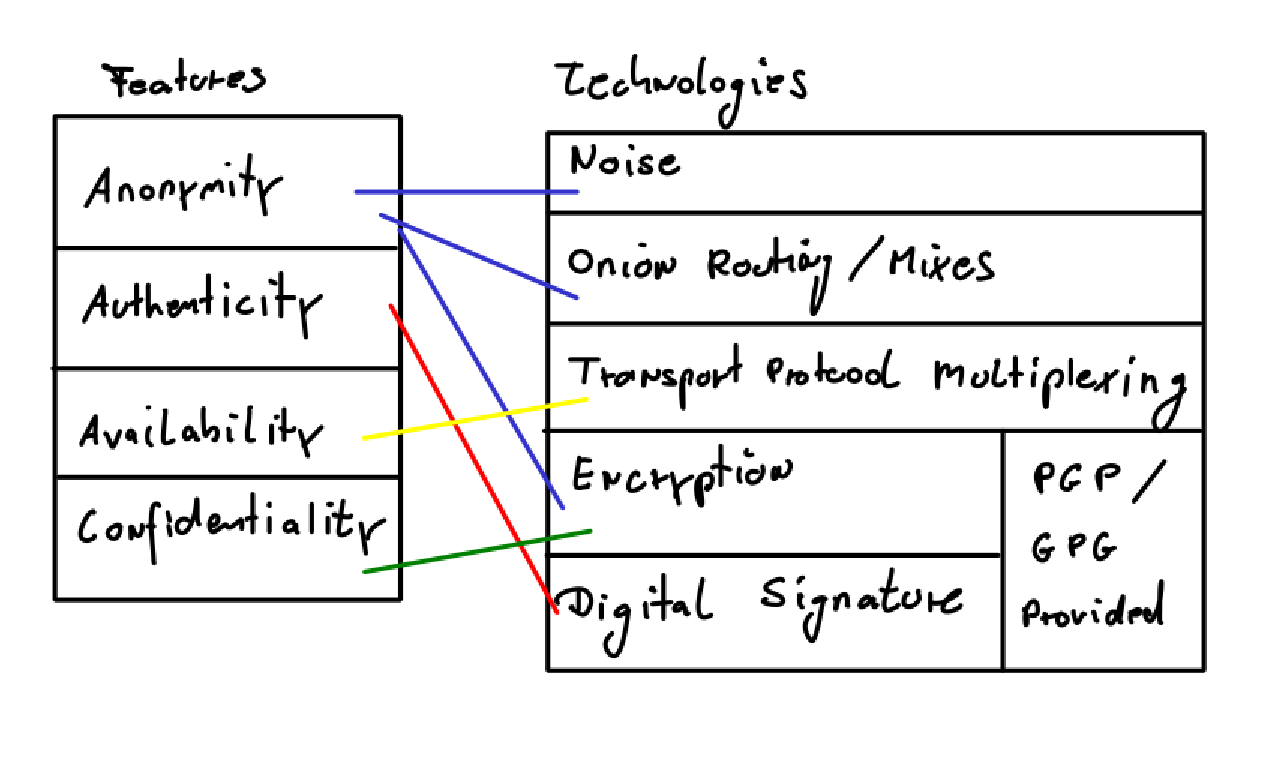
\includegraphics[scale=0.8]{features-technologies.eps}

Im Gegensatz zu den bisherigen Ansätzen stellt diese Arbeit kein vollständiges
Anonymisierungsnetzwerk für allgemeine Dienste bereit, sondern fokussiert auf
den Dienst Chat. Des weiteren wird das Prinzip des resourcenschonenden Arbeitens
bewusst verletzt: Alle Teilnehmer des Netzes versenden kontinuierlich Pakete
um somit statistische Analyse des Netzwerkverkehrs zu vermeiden. Dies hat zur
Folge, dass konstant circa 192 KBit/s der Verbindung durch das Chatsystem
genutzt sind.

Die Anonymisierung wird über eine veränderte Art des Onion Routings sichergestellt.
Im Vergleich zum normalen Onion Routing gibt es in diesem Protokoll keine
externen Endpunkte und der Empfänger kann an beliebiger Stelle der Route
stehen, das Zwiebelpaket wird jedoch immer an eine statische Anzahl von
Peers weitergeleitet. 
Unter Verwendung eines Netzwerkes mit 100 Peers und 5 Proxy Peers kann
so eine Deanonymisierungswahrscheinlichkeit von
1:7.52875e+07 sichergestellt werden, die kleiner ist, als einen 6er im Lotto
zu haben.

\end{document}
